\documentclass[12pt, oneside]{amsart}   	% use "amsart" instead of "article" for AMSLaTeX format
\usepackage[margin=1in]{geometry}                		% See geometry.pdf to learn the layout options. There are lots.
\geometry{letterpaper}                   		% ... or a4paper or a5paper or ... 
%\geometry{landscape}                		% Activate for for rotated page geometry
\usepackage[parfill]{parskip}    		% Activate to begin paragraphs with an empty line rather than an indent
\usepackage{graphicx}				% Use pdf, png, jpg, or eps§ with pdflatex; use eps in DVI mode
								% TeX will automatically convert eps --> pdf in pdflatex		
\usepackage{amssymb,hyperref}
\usepackage{listings}

\title{Week 1: An Introduction to R}
\author{Thomas Elliott}
\date{\today}							% Activate to display a given date or no date

\begin{document}
\maketitle
\lstset{language=R}

\section{Installing R}

The first thing you will want to do if you plan on using R is to install it to your computer. R and official packages for R are maintained on CRAN (Comprehensive R Archive Network), which we will talk about more in week 3. For now, it's enough to know that this is where you go to install R and to download updates to the core R program. You can go to \url{https://cran.r-project.org/} and click on the link appropriate for your operating system to download R. Follow the instructions for installing R and once you are done you should be good to go.

To start R from the command line, open up terminal (or whatever the command line program is called on your operating system), navigate to the folder in which you will be doing your analysis, then type \texttt{R}. This will start R in your command line window. To exit R, you can type \texttt{quit()} or simply \texttt{q()}. R will ask whether to save a copy of your workspace to a hidden data file in the current working directory (more on all of this later --- I rarely say yes to this prompt) and then you will exit back into your command line for your operating system.

\section{Installing RStudio (optional)}

I use R inside of RStudio. RStudio is an IDE (Integrated Development Environment) for R, which means it comes with some extra features that make programming in R, and thus data analysis in R, much easier than working strictly from the command line. Especially if you are new to R, I strongly recommend downloading and installing RStudio as well. RStudio requires R to be installed and is separate from your R install, so you can still use R from the command line even if you install RStudio.

To download RStudio, go to \url{https://www.rstudio.com/products/rstudio/download/} and download the appropriate version for your operating system. Follow the instructions to install the program and once you are done you should be good to go. Just launch RStudio and a session of R will automatically be started in the command line pane of RStudio.

The creators of RStudio also work on a number of packages that make data manipulation much easier than base R (by base R I mean R and those packages automatically loaded when you first start a new R session), as well as a number of other tools that simplify or enhance data analysis. I'll discuss these more as they become relevant, and will try to show how to do something in base R, then show how packages make the process easier. This way, you'll know how it works in base R, but will also know how to save time/code/headache by using relevant packages.

\section{Basics of R}

R, like Stata, is a command line program, meaning you type commands into the command line in order to do things (as opposed to SPSS which is clicking through menus and windows). R's language is more closely related to computer programming languages like C++ and Java than Stata's language, which makes it simultaneously more powerful and more difficult to learn. Let's start with something basic, though: assigning a variable a value.

Assignment in R is done using the \texttt{<-} command:

\begin{lstlisting}
x<-5
\end{lstlisting}

The code above defines a variable called x and assigns the value of 5 to it. You can update x by simply reassigning a new value to it:

\begin{lstlisting}
x<-x+2
\end{lstlisting}

Now x should contain the value 7. You can verify it by typing x into the command line and pressing enter - this will print the contents of the variable to the console:

\begin{lstlisting}
> x
[1] 7
\end{lstlisting}

Nice that \texttt{[1]} that gets outputting before the 7. That's because x is interpreted as a vector of length 1 and 7 is the first value in this vector - we'll talk more about vectors and other data objects later. 

This is a good chance to point out one fundamental difference between Stata and R: Stata often builds in barriers to doing something stupid, for example you have to use replace to change a variable so you don't accidentally over-write a variable with generate. R does not have these same conventions and so it is very easy to over-write data accidentally in R. This means you, as the user, need to be particularly vigilant as you produce your analyses.

We can create a new variable by simply assigning a value to a differently named variable:

\begin{lstlisting}
y<-x-4
> y
[1] 3
\end{lstlisting}

So we assigned the value $x-4$ to y and and then printed the contents of y. This is a good time to talk about the workspace.

\subsection{The Workspace}

In Stata, you open one dataset at a time so your workspace merely consists of the variables in that dataset (plus any matrices or macros you might have created during your session). R, however, allows you to load up multiple datasets into the same workspace, along with many other types of data objects, which I'll describe briefly later and in more detail as the semester goes along. To see a list of all objects currently loaded in the workspace, you can type \texttt{ls()} into the command line and press enter:

\begin{lstlisting}
> ls()
[1] "x" "y"
\end{lstlisting}

So this tells us that there are currently two objects loaded in the workspace, one named x and another named y. This is one area in which RStudio is really helpful. \texttt{ls()} doesn't tell us what x and y are, just that there are objects with those names in our workspace. RStudio, however, has an environment pane that lists all the objects currently loaded in our workspace, plus some additional information about what the objects are and the contents of those objects. Figure \ref{fig:workspace} shows an example of the RStudio workspace pane. You can see that it lists the x and y variables, along with the values contained in those variables.

\begin{figure}[t]
\caption{Workspace Pane of Rstudio}
\label{fig:workspace}
\centering
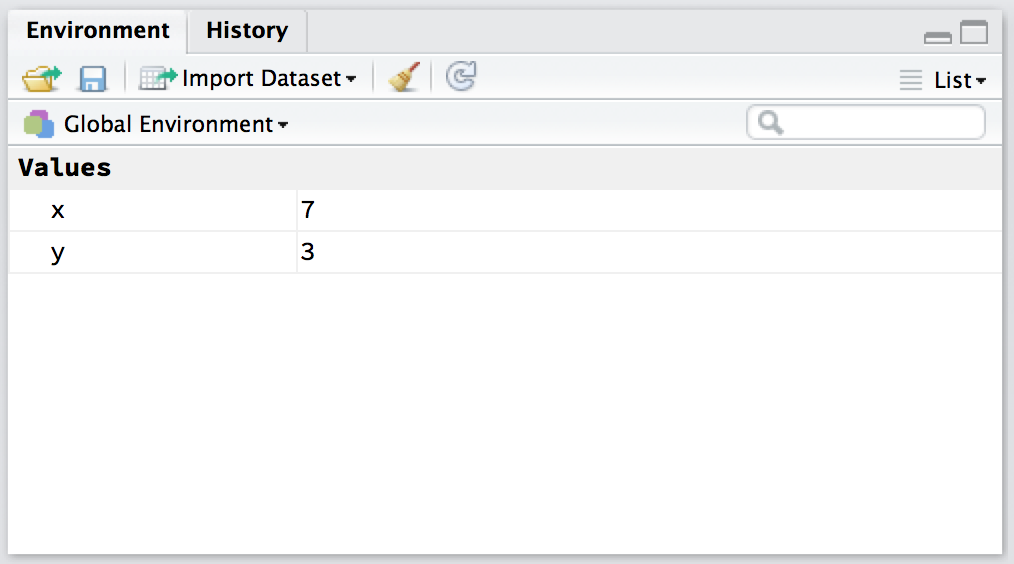
\includegraphics[width=0.75\textwidth]{workspace}
\end{figure}

A more complex example would be a workspace for a project involving some data from my dissertation. Typing \texttt{ls()} provides:

\begin{lstlisting}
> ls()
 [1] "articles"       "claim.talk"     "claims"         "codes"          "exclude"       
 [6] "rangezero"      "smos.data"      "talk.info"      "terms"          "users"         
[11] "yearly.support" "yearly.terms"  
\end{lstlisting}

Whereas RStudio's workspace pane is shown in Figure \ref{fig:workspace2}. RStudio separates out data frames from vectors, arrays, and matrices, and also separately lists out functions. Additional, relevant data is shown for each object. This makes it much easier to organize your workspace and keep track of what you have loaded.

\begin{figure}[t]
\caption{Workspace Pane of RStudio}
\label{fig:workspace2}
\centering
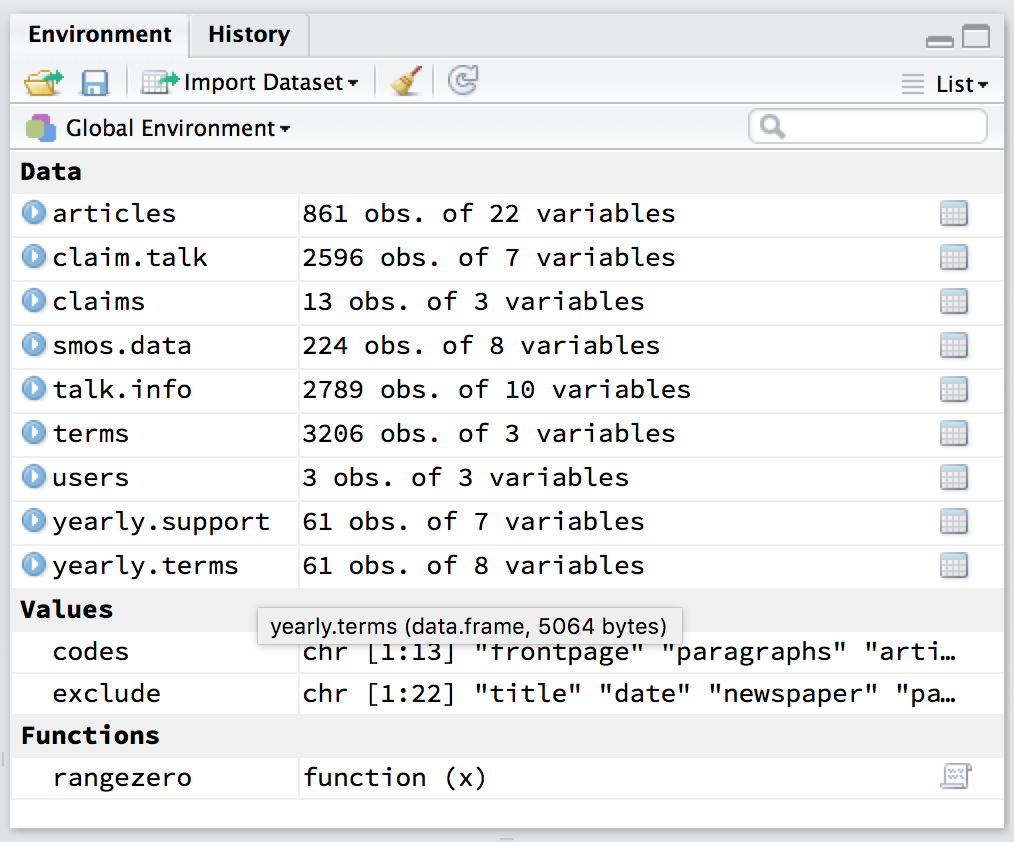
\includegraphics[width=0.75\textwidth]{workspace2}
\end{figure}

R's ability to load multiple, complex data objects into the same workspace is one of the more powerful aspects of R. 

\subsection{Data Objects}

Because R can have multiple data objects loaded at once, there is a greater variety of types of data objects R can work with. I briefly mention the most common types here, and we'll discuss them more as is relevant throughout the semester:

\begin{description}
\item[Data Frames] This is the closest to a data set object R has, and works much like a data set in Stata might work. In a data frame, R assumes that columns are variables and rows are observations. Each column can be a different data type (int, double, string --- more on this later in the semester). Much of the analysis functions (like regression) will ask for a data frame to be passed to it in order to do its analysis, so it will also be the most common data object you will likely work with in R. When you import data from spreadsheets (more on this later in the semester), the data will be saved to a data frame object in your workspace. 
\item[vectors] Vectors are one dimensional groups of values of the same type (int, double, string). As I said earlier, when we assigned x and y above, they were created as vectors of length 1, but you can have vectors of any length (limited by the size of your computer's memory).
\item[matrices and arrays] Arrays are n-dimensional objects containing data entries of the same type (int, double, string). Matrices are two dimensional arrays, and are specially treated in R (meaning there are functions that work only on matrices, not higher-dimensional arrays) since matrices are such common data structures. 
\item[factors] factors are special types of vectors for storing discrete or categorical data. Factors allow labels to be assigned to specific values. The real benefit of factors is that when building a model for a regression, factor variables are automatically dichotomized (equivalent of typing \texttt{i.varname} in Stata) and value labels are used in the regression output. Data frame columns can be factors.
\item[lists] Lists are a special type of vector in which the elements don't need to be the same data type, and are often complex data objects. For example, you could have a list in which three elements are three different data frames, one element is a 4-dimensional array, and one element is yet another list. Lists also have more flexible keys than other objects. Vectors and arrays have automatic numeric indices. Lists allow you to set character keys. We will talk more about keys indices later. Lists are useful for returning the results of statistical analysis - for example, the results from a OLS regression are returned as a list, with various elements containing the coefficients, the residuals, and the significance tests. You are not likely to use lists when you are first getting started with R, but they are very useful objects to be aware of.
\item[functions] user created functions are stored as objects in the R workspace as well. This is important to know, as if you define a function and name it something like \texttt{foo}, then later assign a value to \texttt{foo}, you will have over-written the function. 
\end{description}


\end{document}  